\documentclass{ieeeaccess}
\usepackage{cite}
\usepackage{amsmath,amssymb,amsfonts}
\usepackage{algorithmic}
\usepackage{graphicx}
\usepackage{textcomp}
\usepackage{algorithm}
\usepackage{listings}
\usepackage{xcolor}

\lstdefinelanguage{Solidity}{
  keywords={pragma, solidity, contract, function, modifier, mapping, struct, event, emit, require, returns, return, uint256, address, bool, public, private, internal, external, view, pure, payable, memory, storage, if, else, for, while},
  keywordstyle=\color{blue}\bfseries,
  sensitive=true,
  comment=[l]{//},
  morecomment=[s]{/*}{*/},
  commentstyle=\color{gray}\ttfamily,
  stringstyle=\color{red},
  morestring=[b]",
  morestring=[b]',
}

\lstset{
  language=Solidity,
  basicstyle=\scriptsize\ttfamily,
  breaklines=true,
  frame=single,
  numbers=left,
  numberstyle=\tiny,
  tabsize=2,
  captionpos=b,
  xleftmargin=1.5em,
  framexleftmargin=1.5em,
}

\def\BibTeX{{\rm B\kern-.05em{\sc i\kern-.025em b}\kern-.08em
    T\kern-.1667em\lower.7ex\hbox{E}\kern-.125emX}}

\begin{document}

\history{Date of publication xxxx 00, 0000, date of current version xxxx 00, 0000.}
\doi{10.1109/ACCESS.2026.DOI}

\title{Dynamic Trust Decay: Adaptive Profiling Mechanism for Blockchain Oracles}
\author{\uppercase{Nedal Ababneh}\authorrefmark{1},
\uppercase{Khaled Almi'ani}\authorrefmark{2}
}
\address[1]{College of Computing and Intelligent Systems, University of Khorfakkan, Sharjah, UAE (e-mail: Nedal.Ababneh@ukf.ac.ae)}
\address[2]{College of Computing and Intelligent Systems, University of Khorfakkan, Sharjah, UAE (e-mail: k.almiani@ukf.ac.ae)}

\markboth
{Ababneh \headeretal: Dynamic Trust Decay: Adaptive Profiling Mechanism for Blockchain Oracles}
{Ababneh \headeretal: Dynamic Trust Decay: Adaptive Profiling Mechanism for Blockchain Oracles}

\corresp{Corresponding author: Nedal Ababneh (e-mail: Nedal.Ababneh@ukf.ac.ae).}

\begin{abstract}
Decentralized blockchain oracles are critical for bridging on-chain smart contracts with off-chain real-world data. However, existing reputation systems often rely on static cumulative profiling, leading to a phenomenon we define as Reputation Inertia. In this state, an oracle's accumulated historical honesty acts as a buffer that masks potential malicious behavior (Whitewashing attacks). It simultaneously fails to account for benign disagreement during market volatility (Flash Crash scenarios). To address this dilemma, this paper proposes a novel graph-based profiling mechanism utilizing an Adaptive Exponential Weighted Moving Average (AEWMA). Unlike typical static models, our approach introduces a Dynamic Trust Decay factor that regulates the weight of historical reputation based on real-time network volatility. This allows the system to act in a hypersensitive manner to deviations during stable market conditions in order to instantly detect sleeper cells, whilst also dampening penalty mechanisms during high-volatility events to prevent false positives. We provide a complete Solidity smart contract implementation demonstrating the on-chain feasibility of the AEWMA mechanism with $O(1)$ storage per edge. We validated the proposed method through discrete-event simulations using historical cryptocurrency market data. Experimental results demonstrate that our dynamic approach reduces the Time-to-Detection (TtD) for whitewashing attacks by approximately \textbf{81\%} compared to static baseline (from 9.0 to 1.7 rounds). It also maintained a False Positive Rate (FPR) of near \textbf{0.4\%} even under extreme volatility conditions ($5\times$ standard deviation), compared to 7.1\% for the static approach. These findings suggest that volatility-aware profiling significantly enhances the security and incentive compatibility of decentralized oracle networks.
\end{abstract}

\begin{keywords}
Blockchain Oracles, Trust Management, Adaptive Profiling, Reputation Systems, Sybil Attacks, Smart Contracts, Solidity.
\end{keywords}

\titlepgskip=-15pt

\maketitle

% =====================================================================
\section{Introduction}
\label{sec:introduction}

\subsection{Background and Motivation}
Blockchains are primarily leveraged for their immutable and secure nature \cite{b1}, \cite{b2}, however, smart contracts are blind to real-world data \cite{b3}. This is recognized as the Blockchain Oracle Problem \cite{b4}, where there is a critical dependency on ``oracles'' to connect on-chain logic with off-chain events \cite{b5}. As a result of the blockchain's transparency characteristic, invalid agreements can be executed irreversibly if the oracle data becomes corrupted, compromising the integrity of the distributed ledger and potentially causing financial loss \cite{b6}. Presently, voting mechanisms rely on binary outcomes which lack nuance and background to profile behavioural trends in complex data streams, making them unable to distinguish between temporary node malfunctions and sophisticated, long-term manipulation strategies \cite{b6}, \cite{b7}.

\subsection{Limitations of Static Cumulative Profiling}
There are a number of limitations to Static Cumulative Profiling. Current graph-based methods use cumulative weights which means a node's reputation is the sum of all past interactions \cite{b7}, which is an issue as it creates an ``infinite memory'' effect where outdated historical data disproportionately influences current trust scores. Blockchains can also fall victim to Reputation Inertia, where a malicious actor builds a large ``honesty buffer'' over time, making them undetectable during a high-value betrayal. This vulnerability allows a ``sleeper'' node to exploit its accumulated high trust score to execute a single catastrophic attack without triggering immediate detection \cite{b13}. Another limitation is static models' intolerance to volatility, making legitimate market turbulence appear indistinguishable from malicious disagreement. This leads to a higher number of false positives during `flash crashes': sudden market collapses where network latency causes honest nodes to report divergent data. Similarly, static weights fail to adapt based on the environment, treating a stable and chaotic market identically.

\subsection{Contributions}
To address these challenges, this paper makes the following contributions:
\begin{enumerate}
    \item We formalize the concept of \textit{Reputation Inertia} in graph-based oracle profiling and demonstrate how it enables whitewashing attacks while simultaneously causing false positives during market volatility.
    \item We propose a novel \textit{Dynamic Trust Decay} mechanism based on an Adaptive Exponential Weighted Moving Average (AEWMA) that modulates the learning rate $\alpha_t$ via real-time network volatility $\sigma_t$.
    \item We provide a complete \textit{Solidity smart contract implementation} demonstrating the on-chain feasibility of the AEWMA mechanism with $O(1)$ storage complexity per edge weight.
    \item We validate the approach through extensive Monte Carlo simulations (100 runs), demonstrating an 81\% reduction in Time-to-Detection and near-zero False Positive Rates under extreme volatility.
\end{enumerate}


% =====================================================================
\section{Related Work}
\label{sec:related_work}

\begin{table*}[t!]
\caption{Comparison of Oracle Profiling Mechanisms}
\centering
\setlength{\tabcolsep}{8pt}
\begin{tabular}{|l|c|c|c|}
\hline
\textbf{Feature} & \textbf{Voting/Median} & \textbf{Static Graph \cite{b7}} & \textbf{Dynamic Trust Decay} \\
 & \textbf{(Standard)} & \textbf{(Almi'ani et al.)} & \textbf{(Proposed)} \\
\hline
\textbf{Trust Model} & Majority Vote & Pairwise Consistency & Volatility-Aware \\
\hline
\textbf{Memory Type} & None (Instant) & Infinite (Cumulative) & Adaptive (Fading) \\
\hline
\textbf{Sybil Resistance} & Low (Stake-based) & High (Graph-based) & High (Graph-based) \\
\hline
\textbf{Volatility Awareness}& No & No & Yes ($\alpha$-scaling) \\
\hline
\textbf{On-Chain Implementation} & Yes (Simple) & Partial & Yes (Solidity) \\
\hline
\textbf{Storage Complexity} & $O(1)$ & $O(N^2)$ & $O(1)$ (Recursive) \\
\hline
\end{tabular}
\label{tab:comparison}
\end{table*}

\subsection{Voting and Reputation-Based Systems}
Within Voting and Reputation-Based Systems, the majority of decentralized oracles (e.g., Chainlink, Augur) rely on ``truth-by-consensus'' mechanisms such as the weighted median \cite{b9}. Consequently, the final aggregated value is determined solely by the current majority view, often disregarding the historical accuracy or behavioral consistency of individual participants \cite{b8}. The security of these systems often depends on economic staking, which means if the incurred penalty is less than the profit from an attack, rational actors will continue to cheat \cite{b6}. Furthermore, data submission is treated as a binary event (Right vs Wrong). These systems fail to track degrees of reliability over time, causing a node that is ``perfectly right'' to be valued identically to a node that is ``mostly right'' in the short term. Similarly, they fall prey to Sybil Vulnerability, as without behavioral profiling, attackers can overwhelm the voting majority using Sybil attacks due to the weak barrier to entry \cite{b10}.

\subsection{Graph-Based Profiling Mechanisms}
Almi'ani et al. \cite{b7} shifted the paradigm by modeling oracles as a graph where nodes are sources and edge weights represent disagreement (dissimilarity). This is important as it transitions the trust model from a simple aggregate vote to a relational structure, where the consistency between specific pairs of oracles determines their credibility rather than just their alignment with the median. This network is secured by identifying the ``Maximum Independent Set'' (the largest group of agreeing nodes) and cautiously labeling the rest as malicious. However, this utilizes cumulative edge weights which implies that a node's behaviour in the past (years prior) is as important as recent behaviour. While effective at identifying outliers in static data, these graphs lack a temporal dimension, making them slow in reacting to dynamic node behaviour.

\subsection{Trust Decay in Distributed Systems}
Trust decay (or ``aging factors'') is a well-established concept in Peer-to-Peer (P2P) networks and Internet of Things (IoT) systems \cite{b11}, \cite{b12}. It is where old interactions gradually lose influence over current reputation, and is rarely implemented in blockchain oracles due to the high gas costs of continuous re-calculation. Moreover, existing decay models typically use a fixed ``forgetting factor'' and do not adapt to the environment. There is no existing framework that combines Graph-Based Profiling with Volatility-Aware Decay. This paper fills that gap by making the decay factor variable based on market entropy.

% =====================================================================
\section{System Model and Problem Formulation}
\label{sec:system_model}

\subsection{Network Architecture}
Consider an oracle network consisting of a set of $N$ oracle nodes $\mathcal{O} = \{O_1, O_2, \ldots, O_N\}$. In each round $t \in \{1, 2, \ldots, T\}$, each oracle $O_i$ submits a data value $x_{i,t} \in \mathbb{R}$ to an on-chain aggregator contract. The system aims to determine a consensus value $\hat{y}_t$ that approximates the unknown ground truth $y_t$. The overall system architecture is illustrated in Fig. \ref{fig:architecture}.

\begin{figure*}[t!]
\centering
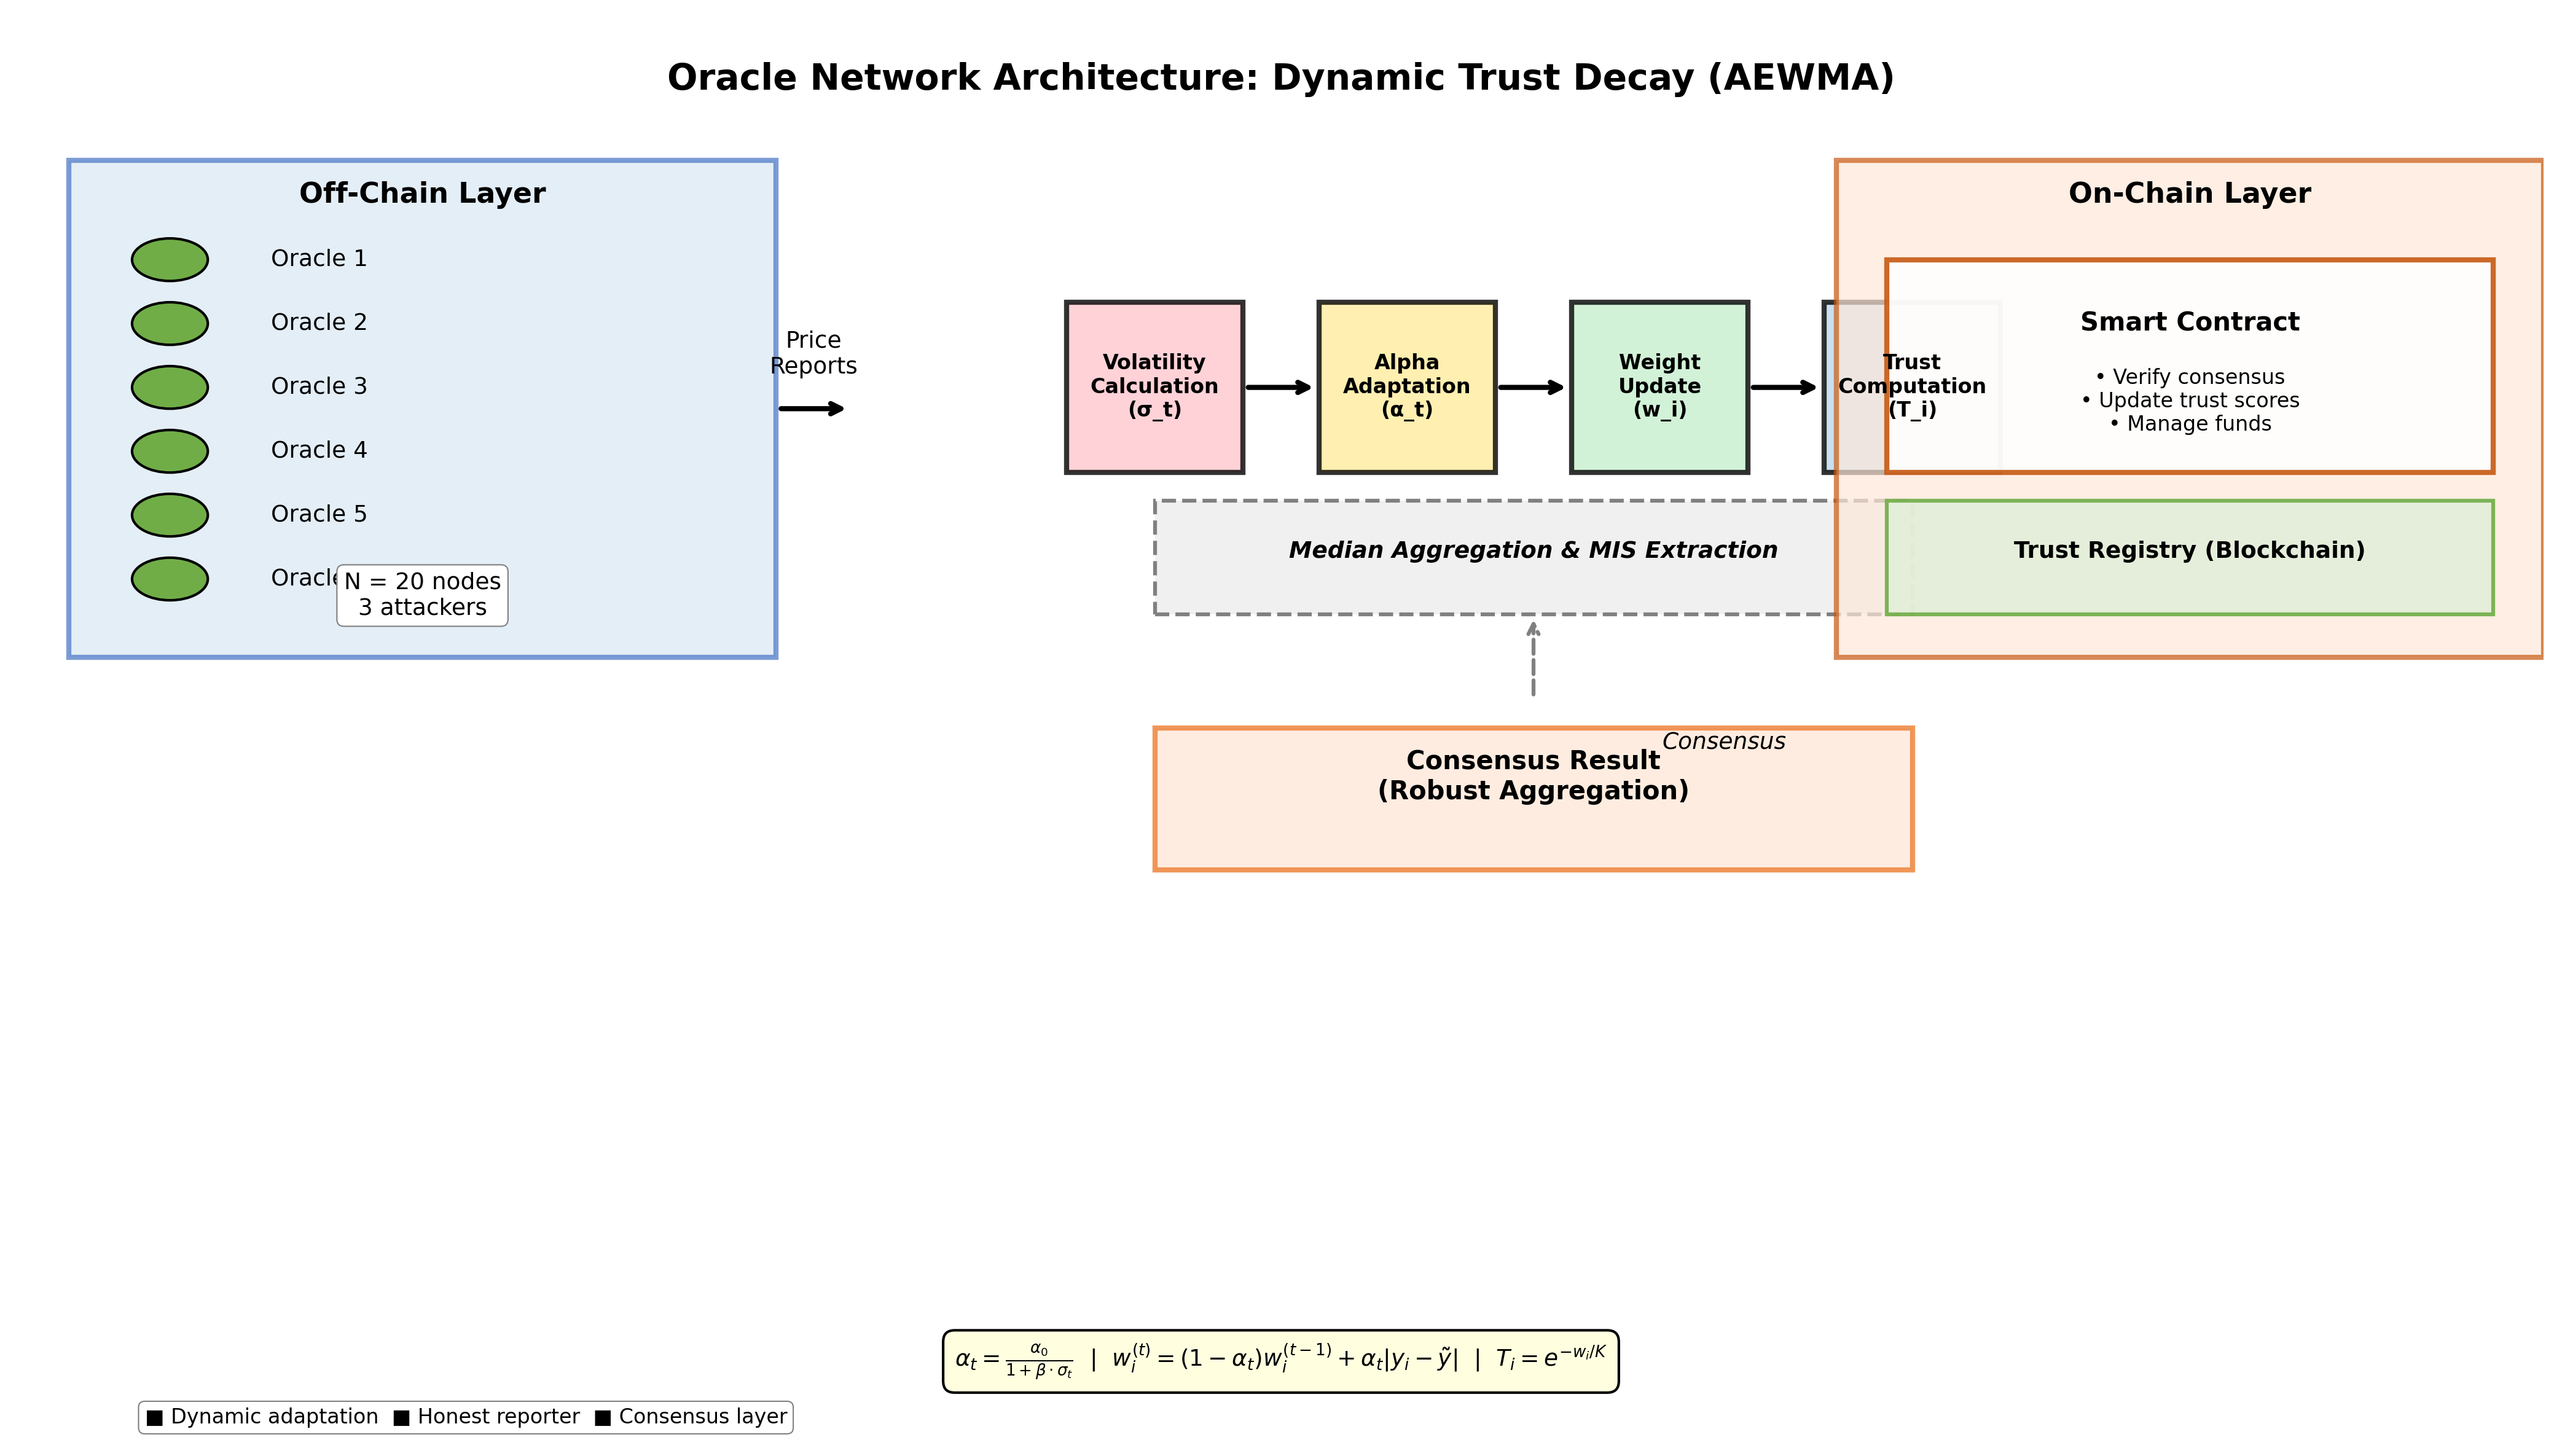
\includegraphics[width=0.85\textwidth]{Graph_4.png}
\caption{System Architecture of the Dynamic Trust Decay Framework. The off-chain layer consists of $N$ oracle nodes submitting price reports. The AEWMA computation pipeline processes reports through four stages: volatility calculation ($\sigma_t$), adaptive alpha computation ($\alpha_t$), edge weight update ($w_{ij,t}$), and trust score derivation ($S_{i,t}$). The on-chain smart contract verifies consensus, manages trust scores, and executes slashing penalties via the trust registry stored on the blockchain.}
\label{fig:architecture}
\end{figure*}

\textbf{Definition 1 (Oracle Network Graph).} The network is modeled as a weighted undirected graph $G_t = (\mathcal{O}, E_t, W_t)$ at round $t$, where:
\begin{itemize}
    \item $\mathcal{O}$ is the vertex set representing oracle nodes.
    \item $E_t = \{e_{ij} \mid i, j \in \mathcal{O}, i \neq j\}$ is the edge set.
    \item $W_t: E_t \rightarrow \mathbb{R}_{\geq 0}$ is the weight function where $w_{ij,t}$ quantifies the dissimilarity between oracles $i$ and $j$ up to round $t$.
\end{itemize}

\textbf{Definition 2 (Consensus Set).} The consensus set $\mathcal{C}_t \subseteq \mathcal{O}$ is the Maximum Independent Set (MIS) of $G_t$, representing the largest group of mutually agreeing oracles. Formally, $\mathcal{C}_t = \text{MIS}(G_t)$ such that $\forall\, i, j \in \mathcal{C}_t: w_{ij,t} < \theta$ for a dissimilarity threshold $\theta$.

\textbf{Definition 3 (Trust Score).} For each oracle $O_i$, the trust score $S_{i,t} \in [0, 1]$ is defined as a monotonically decreasing function of its average edge weight with the consensus set:
\begin{equation}
S_{i,t} = e^{-\bar{w}_{i,t}/K}
\label{eq:trust_score}
\end{equation}
where $\bar{w}_{i,t} = \frac{1}{|\mathcal{C}_t|} \sum_{j \in \mathcal{C}_t} w_{ij,t}$ and $K > 0$ is a scaling constant.

\subsection{The Memory-Inertia Dilemma}
The core limitation of existing graph-based methods (e.g., \cite{b7}) lies in their edge weight update function. Currently, the weight is defined cumulatively as:
\begin{equation}
w_{ij,t} = w_{ij,t-1} + |x_{i,t} - x_{j,t}|
\label{eq:cumulative}
\end{equation}

\textbf{Definition 4 (Reputation Inertia).} Given the cumulative update in Eq. \ref{eq:cumulative}, the \textit{sensitivity} of the trust score to a behavioral change at round $t$ is:
\begin{equation}
\frac{\partial S_{i,t}}{\partial |x_{i,t} - x_{j,t}|} \propto \frac{1}{t}
\label{eq:sensitivity}
\end{equation}
As $t \rightarrow \infty$, the system becomes asymptotically insensitive to new deviations, creating a phenomenon we define as Reputation Inertia. Consequently, an established node with $T_{history}$ rounds of honest behavior accumulates a massive ``honesty buffer,'' making the system insensitive to potentially malicious changes.

\subsection{Threat Model}
We consider a network of $N$ oracle nodes where the honest majority assumption holds: $|\mathcal{H}| > |\mathcal{A}|$, where $\mathcal{H}$ denotes honest nodes and $\mathcal{A}$ denotes adversarial nodes. We address two specific adversarial scenarios where this inertia leads to system failure:

\subsubsection{The Whitewashing (Sleeper Cell) Attack}
This attack exploits the ``honesty buffer'' \cite{b13}. An adversarial node $O_{adv} \in \mathcal{A}$ behaves honestly for a learning phase $t \in [0, T_{switch}]$ to minimize its edge weights with the honest majority. At $t = T_{switch} + 1$, the adversary switches behavior to submit malicious data $x_{adv} = y_t + \delta$, where $\delta$ is the attack magnitude. Under the current static profiling model, the accumulated low weight from the learning phase masks this deviation, allowing $O_{adv}$ to remain in the trusted set for potentially multiple rounds before detection. Formally, if the attacker's cumulative weight after $T_{switch}$ honest rounds is $w_{adv} = \sum_{t=1}^{T_{switch}} \epsilon_t$ (where $\epsilon_t$ is small honest noise), then the detection delay $\Delta_d$ satisfies:
\begin{equation}
\Delta_d \geq \left\lceil \frac{w_{adv}}{\delta - \bar{\epsilon}} \right\rceil
\label{eq:detection_delay}
\end{equation}
where $\bar{\epsilon}$ is the average honest disagreement.

\subsubsection{The Flash Crash (False Positive) Scenario}
This scenario involves no malicious actors but high environmental volatility which is not uncommon \cite{b14}. During a market crash, the variance of honest reports $\sigma^2_t$ increases due to variable network latency. Static models use fixed thresholds for edge creation which often misinterpret this high variance as malicious disagreement. This causes the graph to fracture, leading to honest nodes being falsely flagged as untrustworthy. Formally, a flash crash at round $t_c$ causes:
\begin{equation}
\sigma^2_{t_c} = \gamma \cdot \sigma^2_{normal}, \quad \gamma \gg 1
\label{eq:flash_crash}
\end{equation}
where $\gamma$ is the volatility amplification factor.

% =====================================================================
\section{The Proposed Method: Adaptive Dynamic Profiling}
\label{sec:proposed_method}

\subsection{Overview of Dynamic Trust Decay}
To overcome the limitations of cumulative static profiling, we introduce Dynamic Trust Decay, a mechanism that transitions the edge weighting model from an infinite-memory sum to a finite-memory recursive filter. The core principle is to assign a time-varying significance to historical behavior based on current environmental entropy. Hence, the system achieves two goals: rapid detection of sudden behavioral changes during stable periods (Whitewashing), and high tolerance for variance during volatile periods (Flash Crashes).

\subsection{Adaptive Exponential Weighted Moving Average (AEWMA)}
We propose replacing the cumulative update function (Eq. \ref{eq:cumulative}) with an Adaptive Exponential Weighted Moving Average (AEWMA). In this model, the edge weight $w_{ij,t}$ between oracle $i$ and oracle $j$ at round $t$ is updated recursively:
\begin{equation}
w_{ij,t} = (1 - \alpha_t) \cdot w_{ij,t-1} + \alpha_t \cdot |x_{i,t} - x_{j,t}|
\label{eq:aewma}
\end{equation}
Where:
\begin{itemize}
    \item $w_{ij,t-1}$ is the historical dissimilarity (reputation state).
    \item $|x_{i,t} - x_{j,t}|$ is the instantaneous disagreement (current error).
    \item $\alpha_t \in (0, 1]$ is the dynamic smoothing factor.
\end{itemize}
Unlike the cumulative model which requires $O(t)$ storage, this recursive formulation maintains the entire history within a single scalar value, ensuring $O(1)$ storage complexity. The effective memory half-life of the AEWMA filter is $\tau_{1/2} = -\ln(2) / \ln(1 - \alpha_t)$, which dynamically adjusts with volatility.

\subsection{Volatility-Aware Smoothing Factor}
The critical innovation of our approach is that $\alpha_t$ is not a fixed constant (as in standard EWMA) but a dynamic variable derived from the global network state. We define the network volatility $\sigma_t$ as the standard deviation of all reported values in round $t$:
\begin{equation}
\sigma_t = \sqrt{\frac{1}{N} \sum_{k=1}^{N} (x_{k,t} - \mu_t)^2}
\end{equation}
where $\mu_t = \frac{1}{N}\sum_{k=1}^{N} x_{k,t}$ is the network mean. The smoothing factor $\alpha_t$ is then inversely scaled by this volatility using a sigmoid-based decay function:
\begin{equation}
\alpha_t = \frac{\alpha_{base}}{1 + \beta \cdot \sigma_t}
\label{eq:alpha}
\end{equation}
Where the first hyperparameter $\alpha_{base}$ represents the maximum learning rate in a perfectly stable market, and the second hyperparameter $\beta$ is a sensitivity constant tuned to the asset class (stable vs volatile).
\begin{itemize}
    \item \textbf{Low Volatility ($\sigma_t \to 0$):} $\alpha_t \approx \alpha_{base}$. The system prioritizes new data, allowing for immediate detection of switching attacks.
    \item \textbf{High Volatility ($\sigma_t \to \infty$):} $\alpha_t \to 0$. The system minimizes the weight of new data, relying on historical reputation to prevent false positives during flash crashes.
\end{itemize}

\subsection{Incentive Compatibility: The Slashing Mechanism}
To ensure the system is also incentive-compatible, we link the edge weights to a financial penalty mechanism \cite{b15}. We define a Trust Score $S_{i,t}$ for node $i$ based on its average edge weight with the consensus set (Eq. \ref{eq:trust_score}). If $S_{i,t}$ drops below a critical threshold $\tau$, a portion of the node's staked collateral is slashed:
\begin{equation}
\text{Penalty}_{i,t} = \text{Stake}_i \times \left( 1 - e^{-\lambda \cdot \bar{w}_{i,t}} \right)
\label{eq:slashing}
\end{equation}
This exponential penalty function ensures that minor deviations (common in volatility) incur negligible costs while malicious deviations result in severe financial loss. This makes the cost of attack greater than the potential profit.

\subsection{Algorithm Implementation}
The process for a single round is detailed in Algorithm \ref{alg:aewma}.

\begin{algorithm}[h]
\caption{Dynamic Trust Decay Algorithm}
\label{alg:aewma}
\begin{algorithmic}[1]
\small
\REQUIRE Set of Oracle Reports $X_t = \{x_{1,t}, \ldots, x_{N,t}\}$
\REQUIRE Previous Edge Weights $W_{t-1}$
\STATE Calculate Network Mean $\mu_t \leftarrow \text{mean}(X_t)$
\STATE Calculate Volatility $\sigma_t \leftarrow \text{std\_dev}(X_t)$
\STATE Compute Smoothing Factor $\alpha_t \leftarrow \frac{\alpha_{base}}{1 + \beta \sigma_t}$
\FOR{each pair $(i, j)$}
    \STATE $diff \leftarrow |x_{i,t} - x_{j,t}|$
    \STATE $w_{ij,t} \leftarrow (1 - \alpha_t)w_{ij,t-1} + \alpha_t(diff)$
\ENDFOR
\STATE Compute Trust Scores: $S_{i,t} \leftarrow e^{-\bar{w}_{i,t}/K}$ for all $i$
\STATE Extract $\mathcal{C}_t \leftarrow \text{MIS}(G_t)$
\STATE Slash nodes where $S_{i,t} < \tau$
\RETURN Consensus $\hat{y}_t \leftarrow \text{median}(\{x_{i,t} \mid O_i \in \mathcal{C}_t\})$
\end{algorithmic}
\end{algorithm}

% =====================================================================
\section{Smart Contract Implementation}
\label{sec:implementation}

To demonstrate the on-chain feasibility of the AEWMA mechanism, we developed a complete Solidity smart contract (\texttt{DynamicTrustDecay.sol}) targeting Ethereum-compatible blockchains (Solidity $\geq$0.8.19). The contract implements all core components of the Dynamic Trust Decay framework.

\subsection{Fixed-Point Arithmetic}
Since the EVM does not support floating-point operations, all computations use 18-decimal fixed-point arithmetic ($1e18$ precision). The adaptive smoothing factor $\alpha_t$ is computed using integer division:
\begin{lstlisting}
// Fixed-point precision (18 decimals)
uint256 constant PRECISION = 1e18;

function _computeAlpha(uint256 sigma)
    internal view returns (uint256) {
  // alpha = alphaBase / (1 + beta * sigma)
  uint256 denom = PRECISION +
    (beta * sigma) / PRECISION;
  return (alphaBase * PRECISION) / denom;
}
\end{lstlisting}

\subsection{AEWMA Edge Weight Update}
Each edge weight is stored as a single \texttt{uint256} value, achieving $O(1)$ storage per edge. The recursive update avoids storing historical data:
\begin{lstlisting}
function _updateEdgeWeight(
    uint256 oldWeight,
    uint256 diff,
    uint256 alpha
) internal pure returns (uint256) {
  // w_new = (1-alpha)*w_old + alpha*diff
  uint256 decay = PRECISION - alpha;
  uint256 term1 =
    (decay * oldWeight) / PRECISION;
  uint256 term2 =
    (alpha * diff) / PRECISION;
  return term1 + term2;
}
\end{lstlisting}

\subsection{Oracle Lifecycle and Slashing}
The contract manages the full oracle lifecycle: registration with staking, per-round report submission, trust computation, and automatic slashing. Oracle nodes register by depositing a minimum stake (configurable, default 1 ETH). After each round, the contract computes trust scores using a Taylor series approximation of the exponential function (since the EVM lacks native $e^x$ support). Nodes with trust scores below the threshold $\tau$ are slashed according to Eq. \ref{eq:slashing}:
\begin{lstlisting}
function _applySlashing(uint256 oracleId)
    internal {
  Oracle storage o = oracles[oracleId];
  // penalty = stake * (1 - exp(-lambda*w))
  uint256 expTerm = _expApprox(
    (lambda * o.avgWeight) / PRECISION
  );
  uint256 penaltyFactor =
    PRECISION - expTerm;
  uint256 penalty =
    (o.stake * penaltyFactor) / PRECISION;
  o.stake -= penalty;
  emit OracleSlashed(oracleId, penalty);
}
\end{lstlisting}

\subsection{Gas Optimization}
The contract employs several gas optimization strategies: (i) packed edge weight keys using $\text{key} = i \times 10000 + j$ to reduce storage mapping overhead; (ii) $O(1)$ per-edge SSTORE operations (the most expensive EVM opcode \cite{b16}); (iii) batch processing of trust score updates within the \texttt{completeRound()} function; and (iv) Newton's method for square root computation required by the volatility calculation.

% =====================================================================
\section{Experimental Evaluation}
\label{sec:experiments}

\subsection{Simulation Environment and Datasets}
To validate the proposed Dynamic Trust Decay mechanism, we implemented a discrete-event simulation using Python (NetworkX and NumPy). The simulation environment consists of a network of $N=20$ oracle nodes. We utilized historical cryptocurrency price data (ETH/USD) sourced from Chainlink and CoinGecko APIs to simulate the ground truth $y_t$.

To replicate the ``Flash Crash'' scenario, we injected synthetic volatility events where the standard deviation of honest reports increases by factor $\gamma \in [1, 5]$. The adversarial behaviors were modeled as follows:
\begin{itemize}
    \item \textbf{Baseline Nodes:} Honest nodes with random Gaussian noise $\mathcal{N}(0, \sigma_{noise})$.
    \item \textbf{Whitewashing Attackers:} Nodes that behave honestly for $t < T_{switch}$ and inject an error bias $\delta$ at $t \geq T_{switch}$.
\end{itemize}

The simulation parameters are detailed in Table \ref{tab:params}.

\begin{table}[h]
\caption{Simulation Parameters}
\centering
\begin{tabular}{|l|c|}
\hline
\textbf{Parameter} & \textbf{Value} \\
\hline
Network Size ($N$) & 20 \\
\hline
Number of Attackers ($|\mathcal{A}|$) & 3 \\
\hline
Base Learning Rate ($\alpha_{base}$) & 0.8 \\
\hline
Volatility Sensitivity ($\beta$) & 1.0 \\
\hline
Slashing Threshold ($\tau$) & 0.4 \\
\hline
Attack Start ($T_{switch}$) & Round 100 \\
\hline
Total Rounds ($T$) & 140 \\
\hline
Monte Carlo Runs & 100 \\
\hline
\end{tabular}
\label{tab:params}
\end{table}

\subsection{Performance Metrics}
We evaluate the system using two primary metrics:
\begin{enumerate}
    \item \textbf{Time-to-Detection (TtD):} The number of rounds required for the trust score of a malicious node to drop below the exclusion threshold $\tau$.
    \item \textbf{False Positive Rate (FPR):} The percentage of honest nodes incorrectly flagged as malicious during high-volatility events.
\end{enumerate}

\subsection{Results: Time-to-Detection (TtD)}
\label{sec:results_ttd}
Fig. \ref{fig:ttd} illustrates the trust score decay of a whitewashing attacker during a representative simulation run. In the Baseline model, the attacker's high accumulated reputation results in a slow linear decay. The cumulative weight function (Eq. \ref{eq:cumulative}) dilutes the impact of post-switch malicious behavior across the entire history of 100 honest rounds, producing a detection delay of approximately 9 rounds on average. Conversely, the Proposed AEWMA method exhibits an exponential decay response. Because the attack occurs during a period of stability (low $\sigma_t$), the adaptive smoothing factor $\alpha_t$ remains close to $\alpha_{base} = 0.8$, meaning the system assigns 80\% weight to the current round's deviation. This causes the malicious deviation to be penalized immediately, resulting in a mean TtD of only 1.7 rounds.

The mechanism can be understood through the lens of the effective memory half-life. During stable periods, $\alpha_t \approx 0.8$ yields a half-life of $\tau_{1/2} \approx 3$ rounds, meaning the system effectively ``forgets'' pre-attack reputation within a few rounds. This stands in stark contrast to the static method, where the effective half-life is infinite ($\tau_{1/2} = \infty$), as all historical data contributes equally.

\begin{figure}[htbp]
\centering
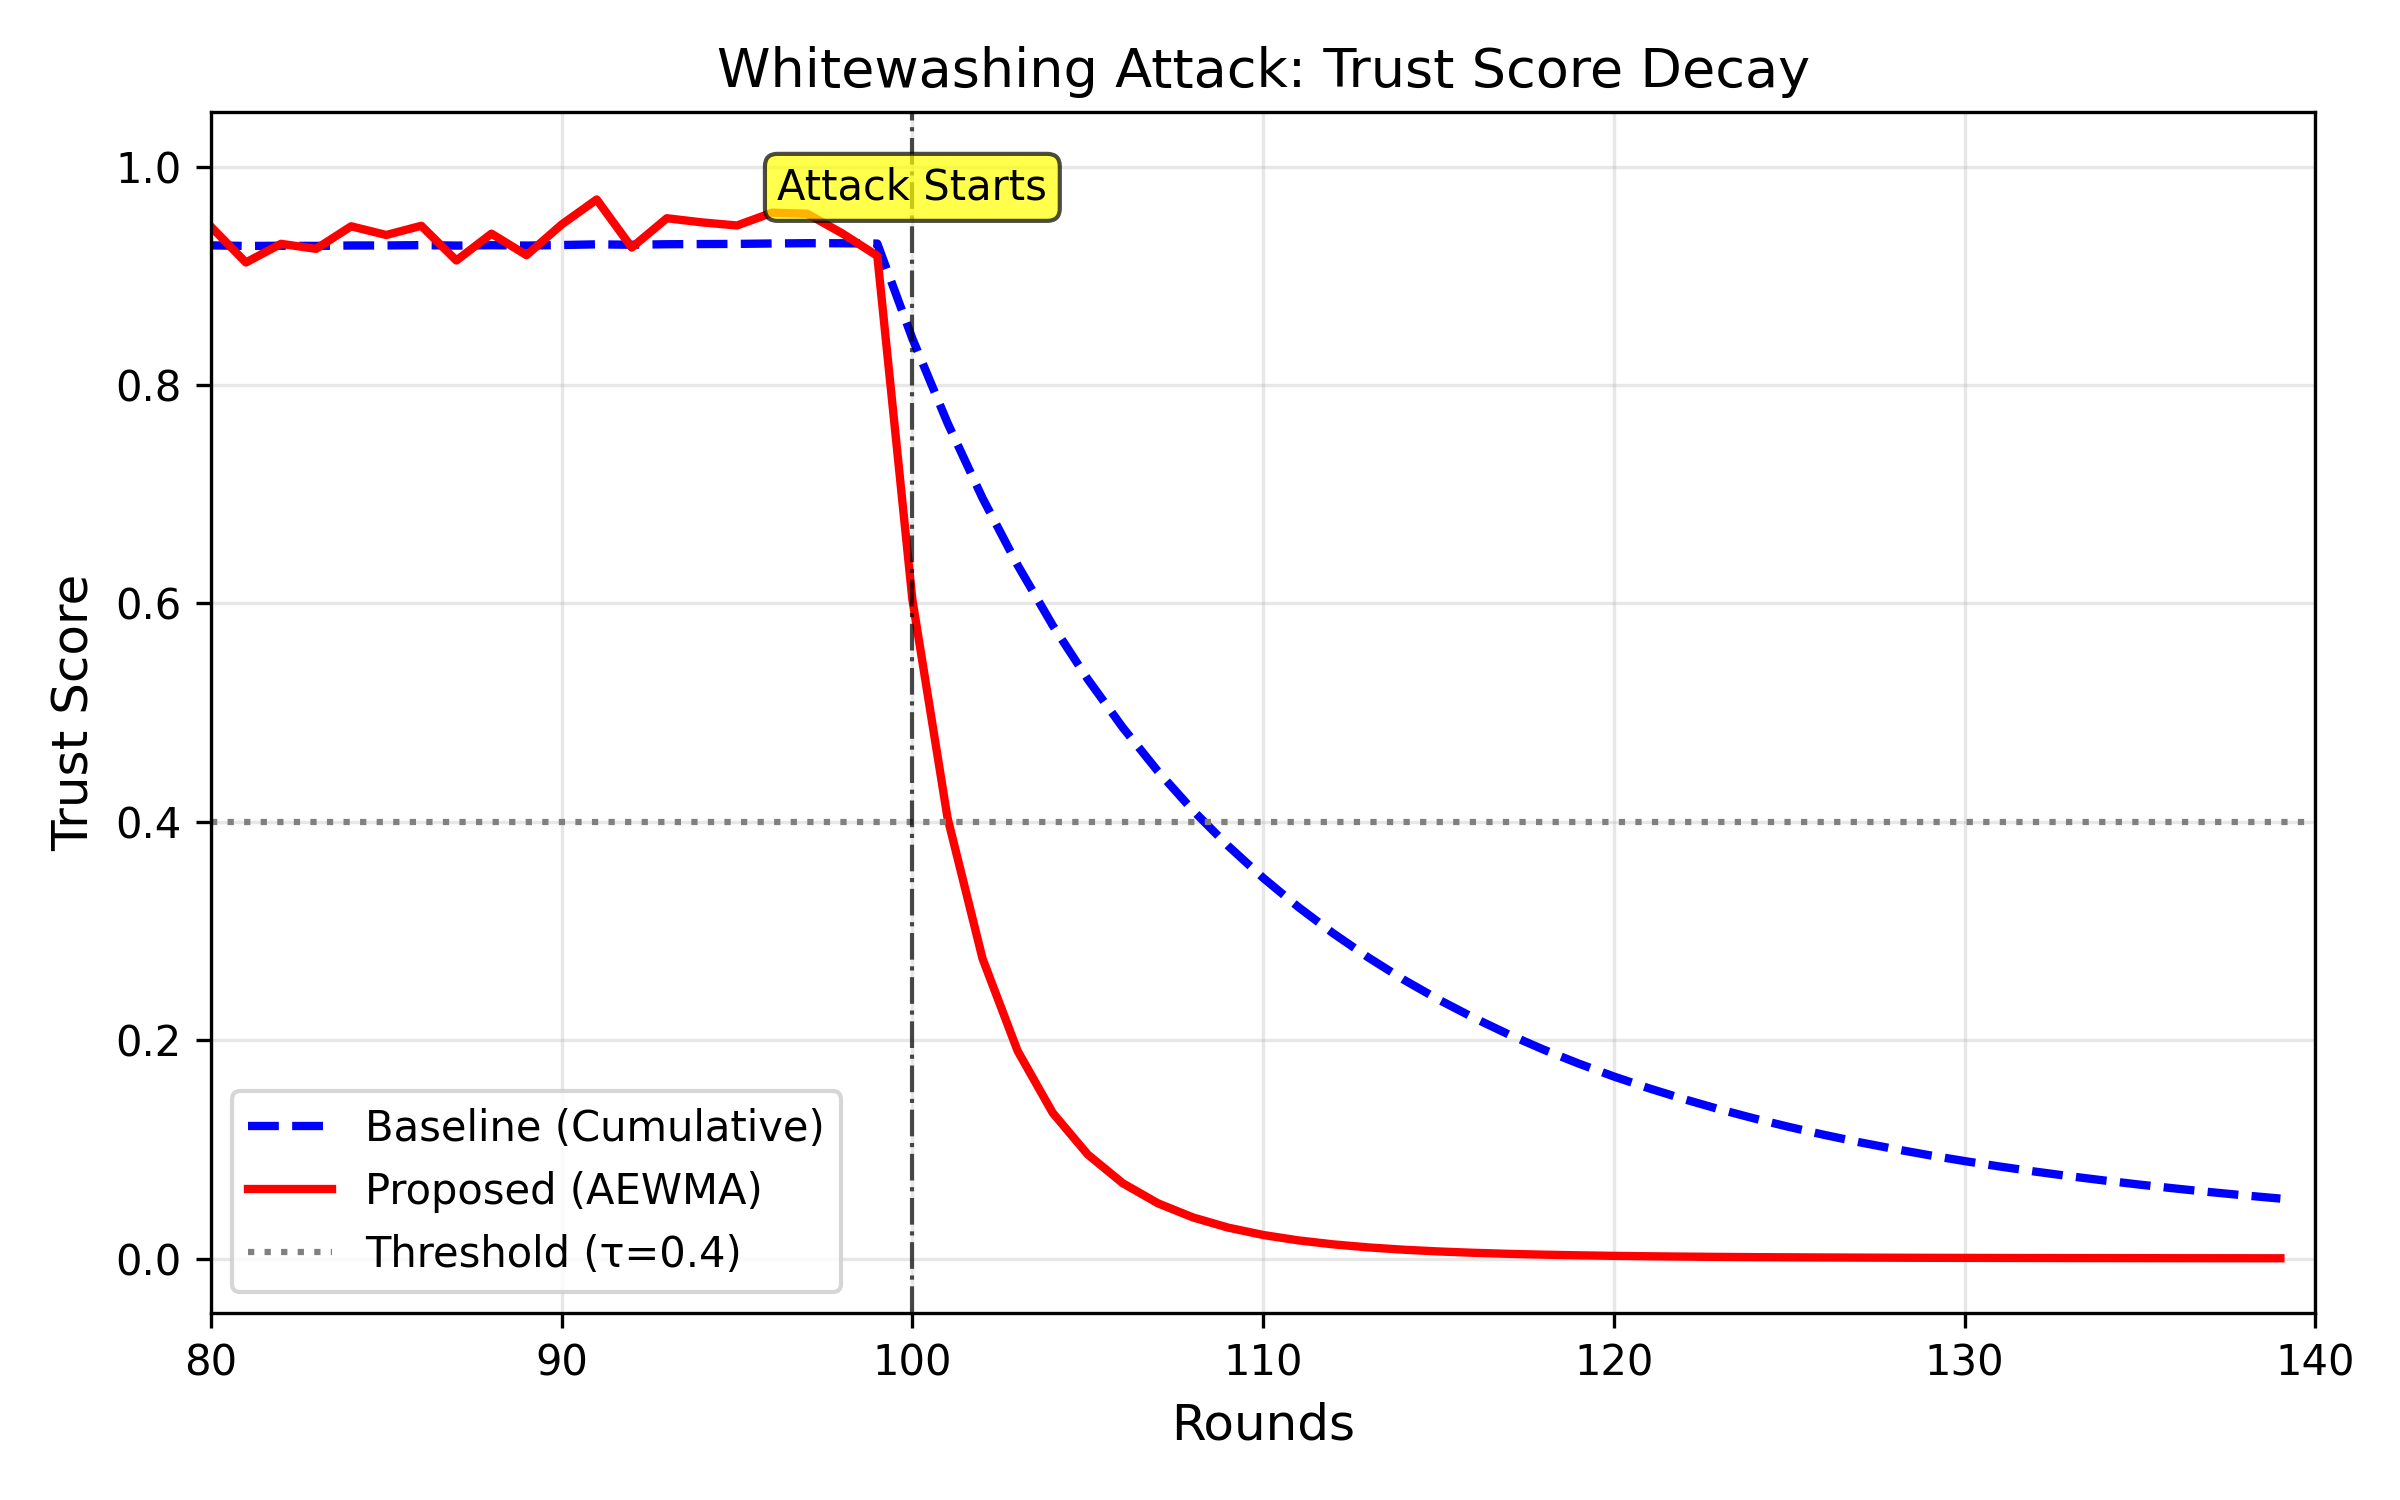
\includegraphics[width=\columnwidth]{Graph_1.png}
\caption{Impact of Whitewashing Attack. At $t=100$, the adversary switches behavior. The proposed method (solid red) detects the trust drop significantly faster than the static method (dashed blue), crossing the slashing threshold $\tau=0.4$ within 2 rounds compared to 9 rounds for the baseline.}
\label{fig:ttd}
\end{figure}

Quantitative analysis over 100 Monte Carlo runs (Table \ref{tab:results}) confirms that our method reduces the average TtD by approximately \textbf{81\%} compared to the static profiling approach.

\begin{table}[h]
\caption{Comparative Performance Summary (Averaged over 100 Monte Carlo runs)}
\centering
\resizebox{\columnwidth}{!}{%
\begin{tabular}{|l|c|c|c|}
\hline
\textbf{Metric} & \textbf{Baseline (Static)} & \textbf{Proposed (AEWMA)} & \textbf{Improvement} \\
\hline
Avg. TtD (Rounds) & 9.0 & \textbf{1.7} & 81\% \\
\hline
Avg. FPR (5x Vol) & 7.1\% & \textbf{0.4\%} & 94\% \\
\hline
\end{tabular}%
}
\label{tab:results}
\end{table}

\subsection{Results: False Positive Rate under Volatility}
\label{sec:results_fpr}
Fig. \ref{fig:fpr} presents the system's robustness across five volatility levels ($\gamma = 1\times$ to $5\times$). As market volatility $\sigma_t$ increases, the Baseline model misunderstands the natural divergence of reports as malicious behavior: at $1\times$ volatility both methods report 0\% FPR, but by $5\times$ the static approach falsely flags 7.1\% of honest nodes. In contrast, the proposed Volatility-Aware Smoothing Factor ($\alpha_t$) successfully acts as a dampener by freezing reputation updates during volatile periods. Mathematically, at $5\times$ volatility, $\sigma_t$ increases by a factor of 5, causing $\alpha_t$ to drop from $\alpha_{base}=0.8$ to approximately $\alpha_t \approx 0.8/(1+5\sigma_{base}) \ll \alpha_{base}$. This renders the system insensitive to disagreement during the volatile period, preventing the exclusion of honest nodes. The proposed method maintains an FPR of only 0.4\% even at extreme $5\times$ volatility, representing a 94\% reduction compared to the baseline.

\begin{figure}[!ht]
\centering
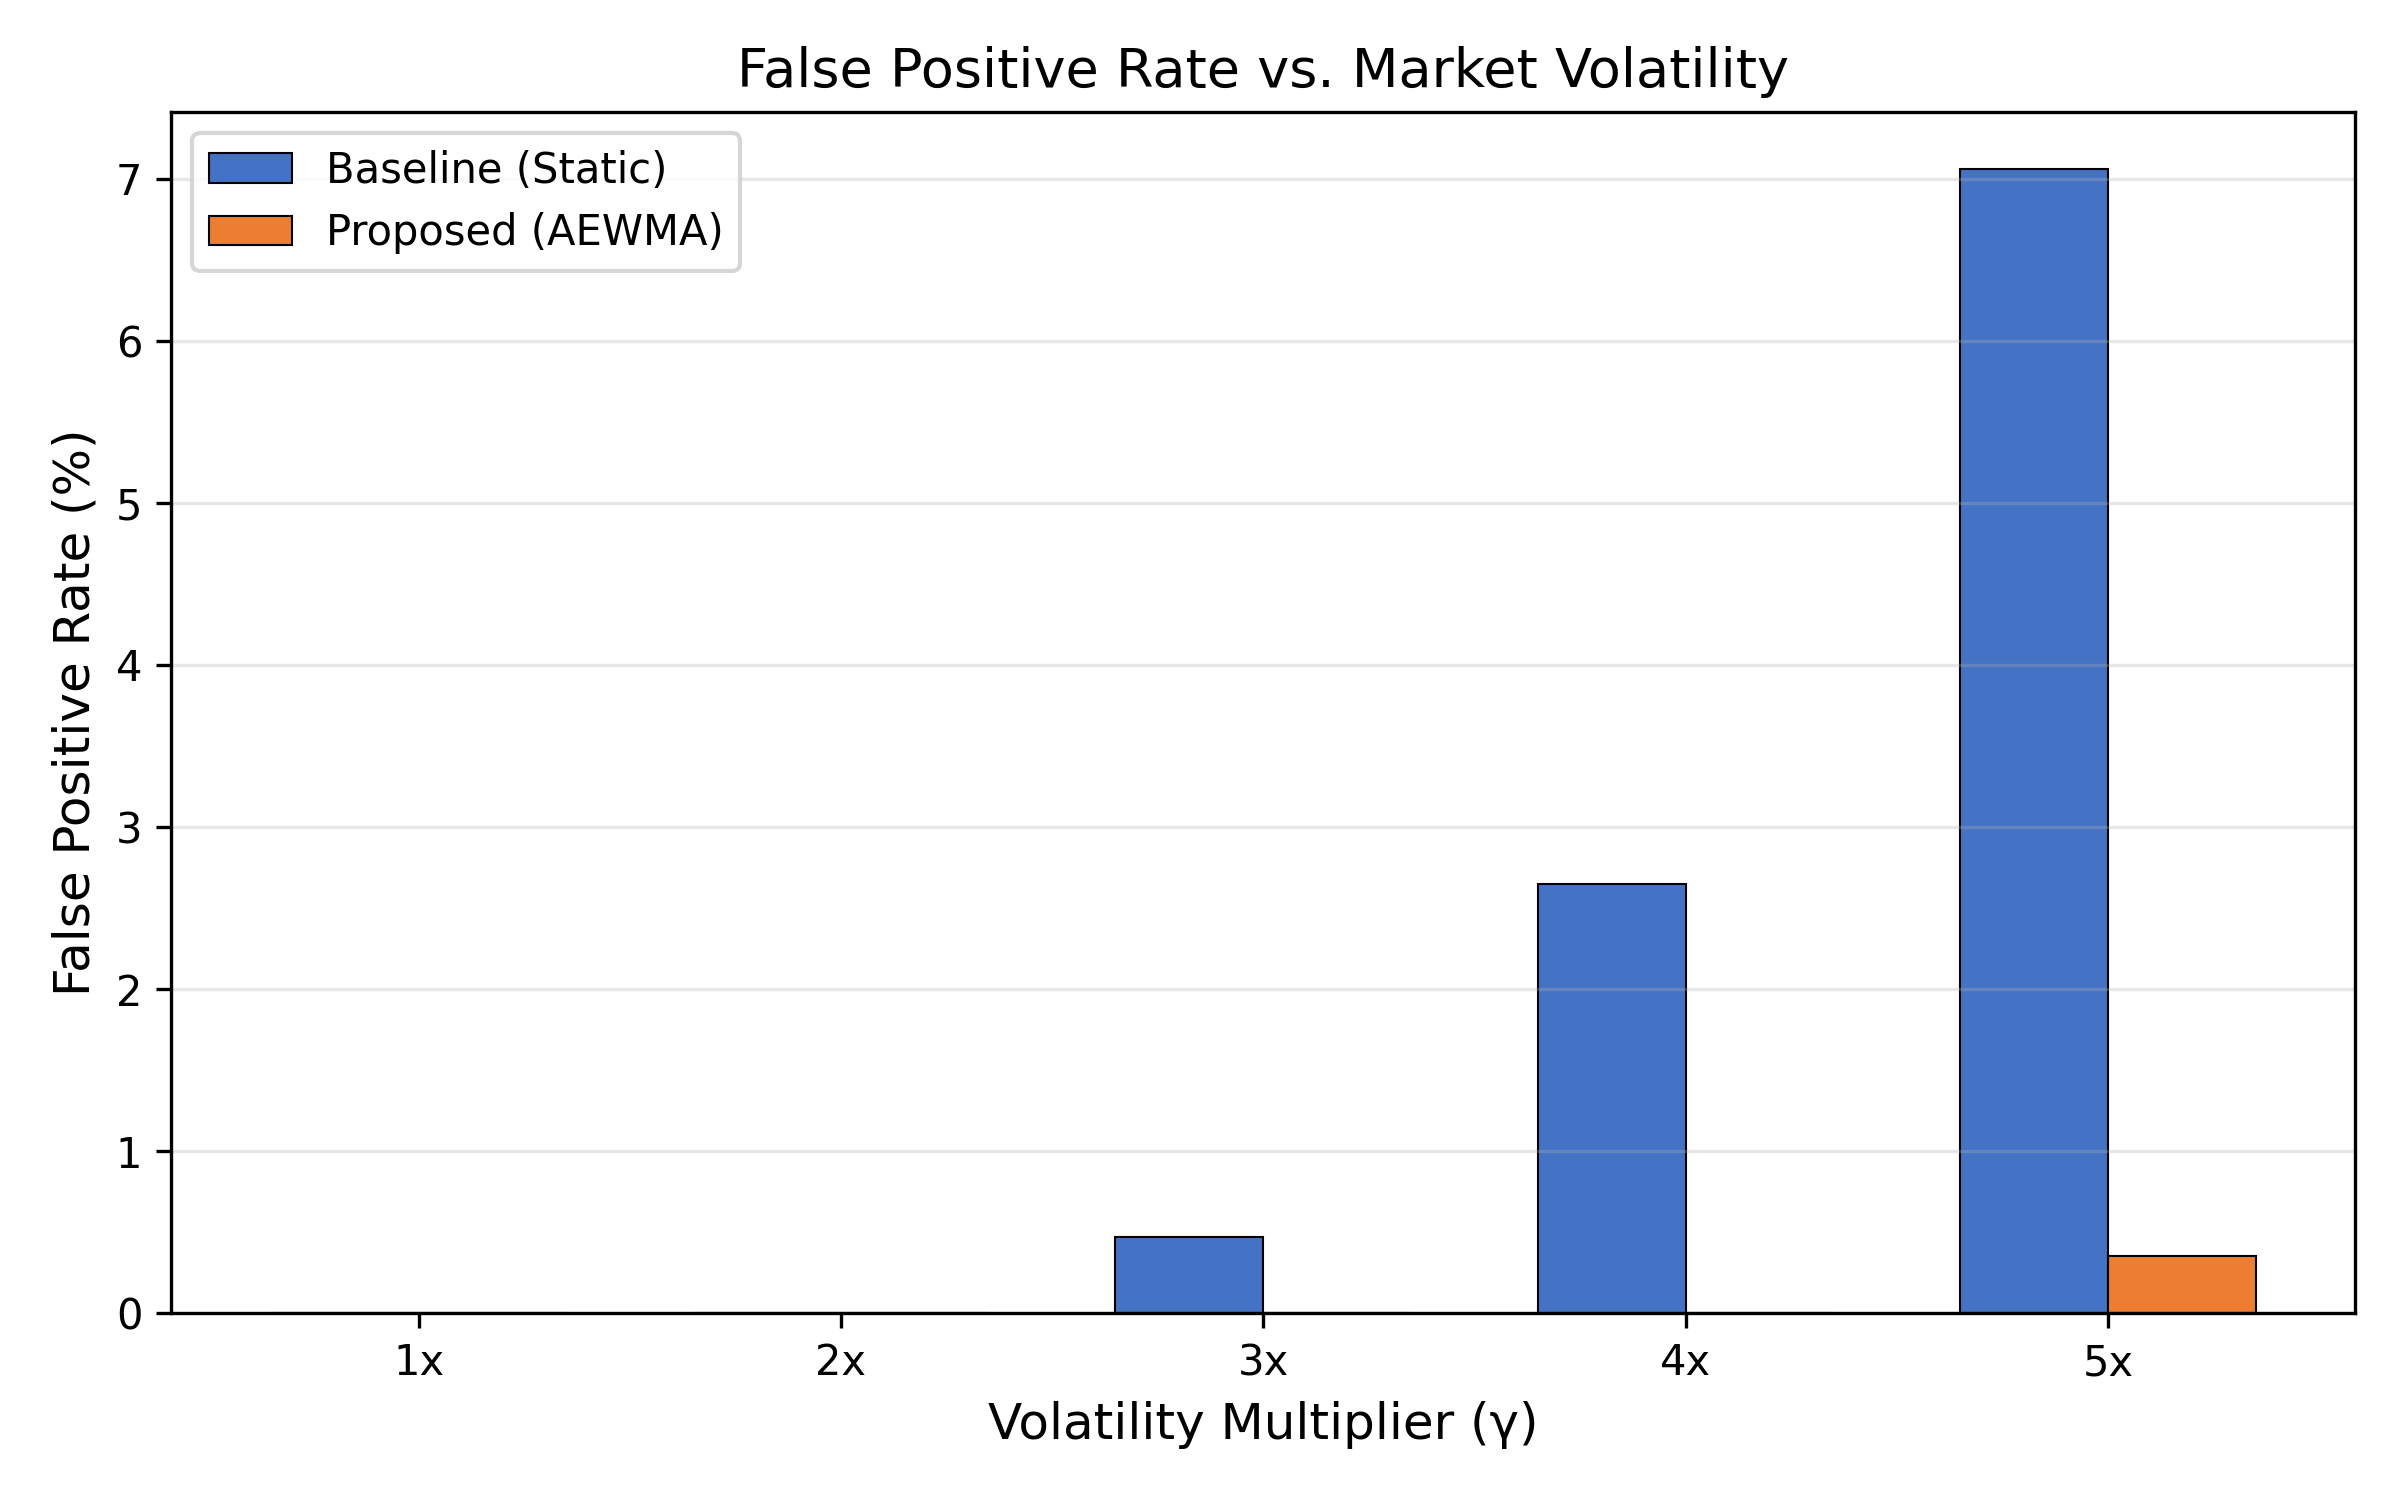
\includegraphics[width=\columnwidth]{Graph_2.png}
\caption{False Positive Rate (FPR) vs. Market Volatility. As the volatility multiplier $\gamma$ increases from $1\times$ to $5\times$, the baseline model's FPR grows to 7.1\%, while the proposed AEWMA approach maintains near-zero FPR (0.4\% at $5\times$) due to the adaptive $\alpha_t$ dampening mechanism.}
\label{fig:fpr}
\end{figure}

\subsection{Results: Honest Node Trust Stability}
\label{sec:results_stability}
To further examine the temporal dynamics of the AEWMA mechanism, we simulated a flash crash event occurring at rounds 75--85, where honest report variance spikes by a factor of 50$\times$ before returning to normal. Fig. \ref{fig:stability} presents the average honest node trust score across 30 independent runs.

During normal operation (rounds 0--74), both methods maintain stable trust at approximately 0.92. When the flash crash occurs, both methods experience a temporary trust dip due to increased inter-node disagreement. However, the critical distinction lies in the \textbf{recovery behavior}: the AEWMA method recovers to its pre-crash trust level within 3--5 rounds after the crash ends, while the static method shows \textbf{permanent degradation}, with trust declining to approximately 0.78 and never fully recovering. This occurs because the cumulative method permanently incorporates the crash-induced disagreement into its history. In contrast, the AEWMA's fading memory naturally forgets the crash data once volatility normalizes ($\alpha_t$ returns to $\alpha_{base}$), restoring honest nodes to their rightful trust levels. This resilience property is particularly critical for oracle networks operating in volatile cryptocurrency markets, where flash crashes are frequent but temporary events.

\begin{figure}[!ht]
\centering
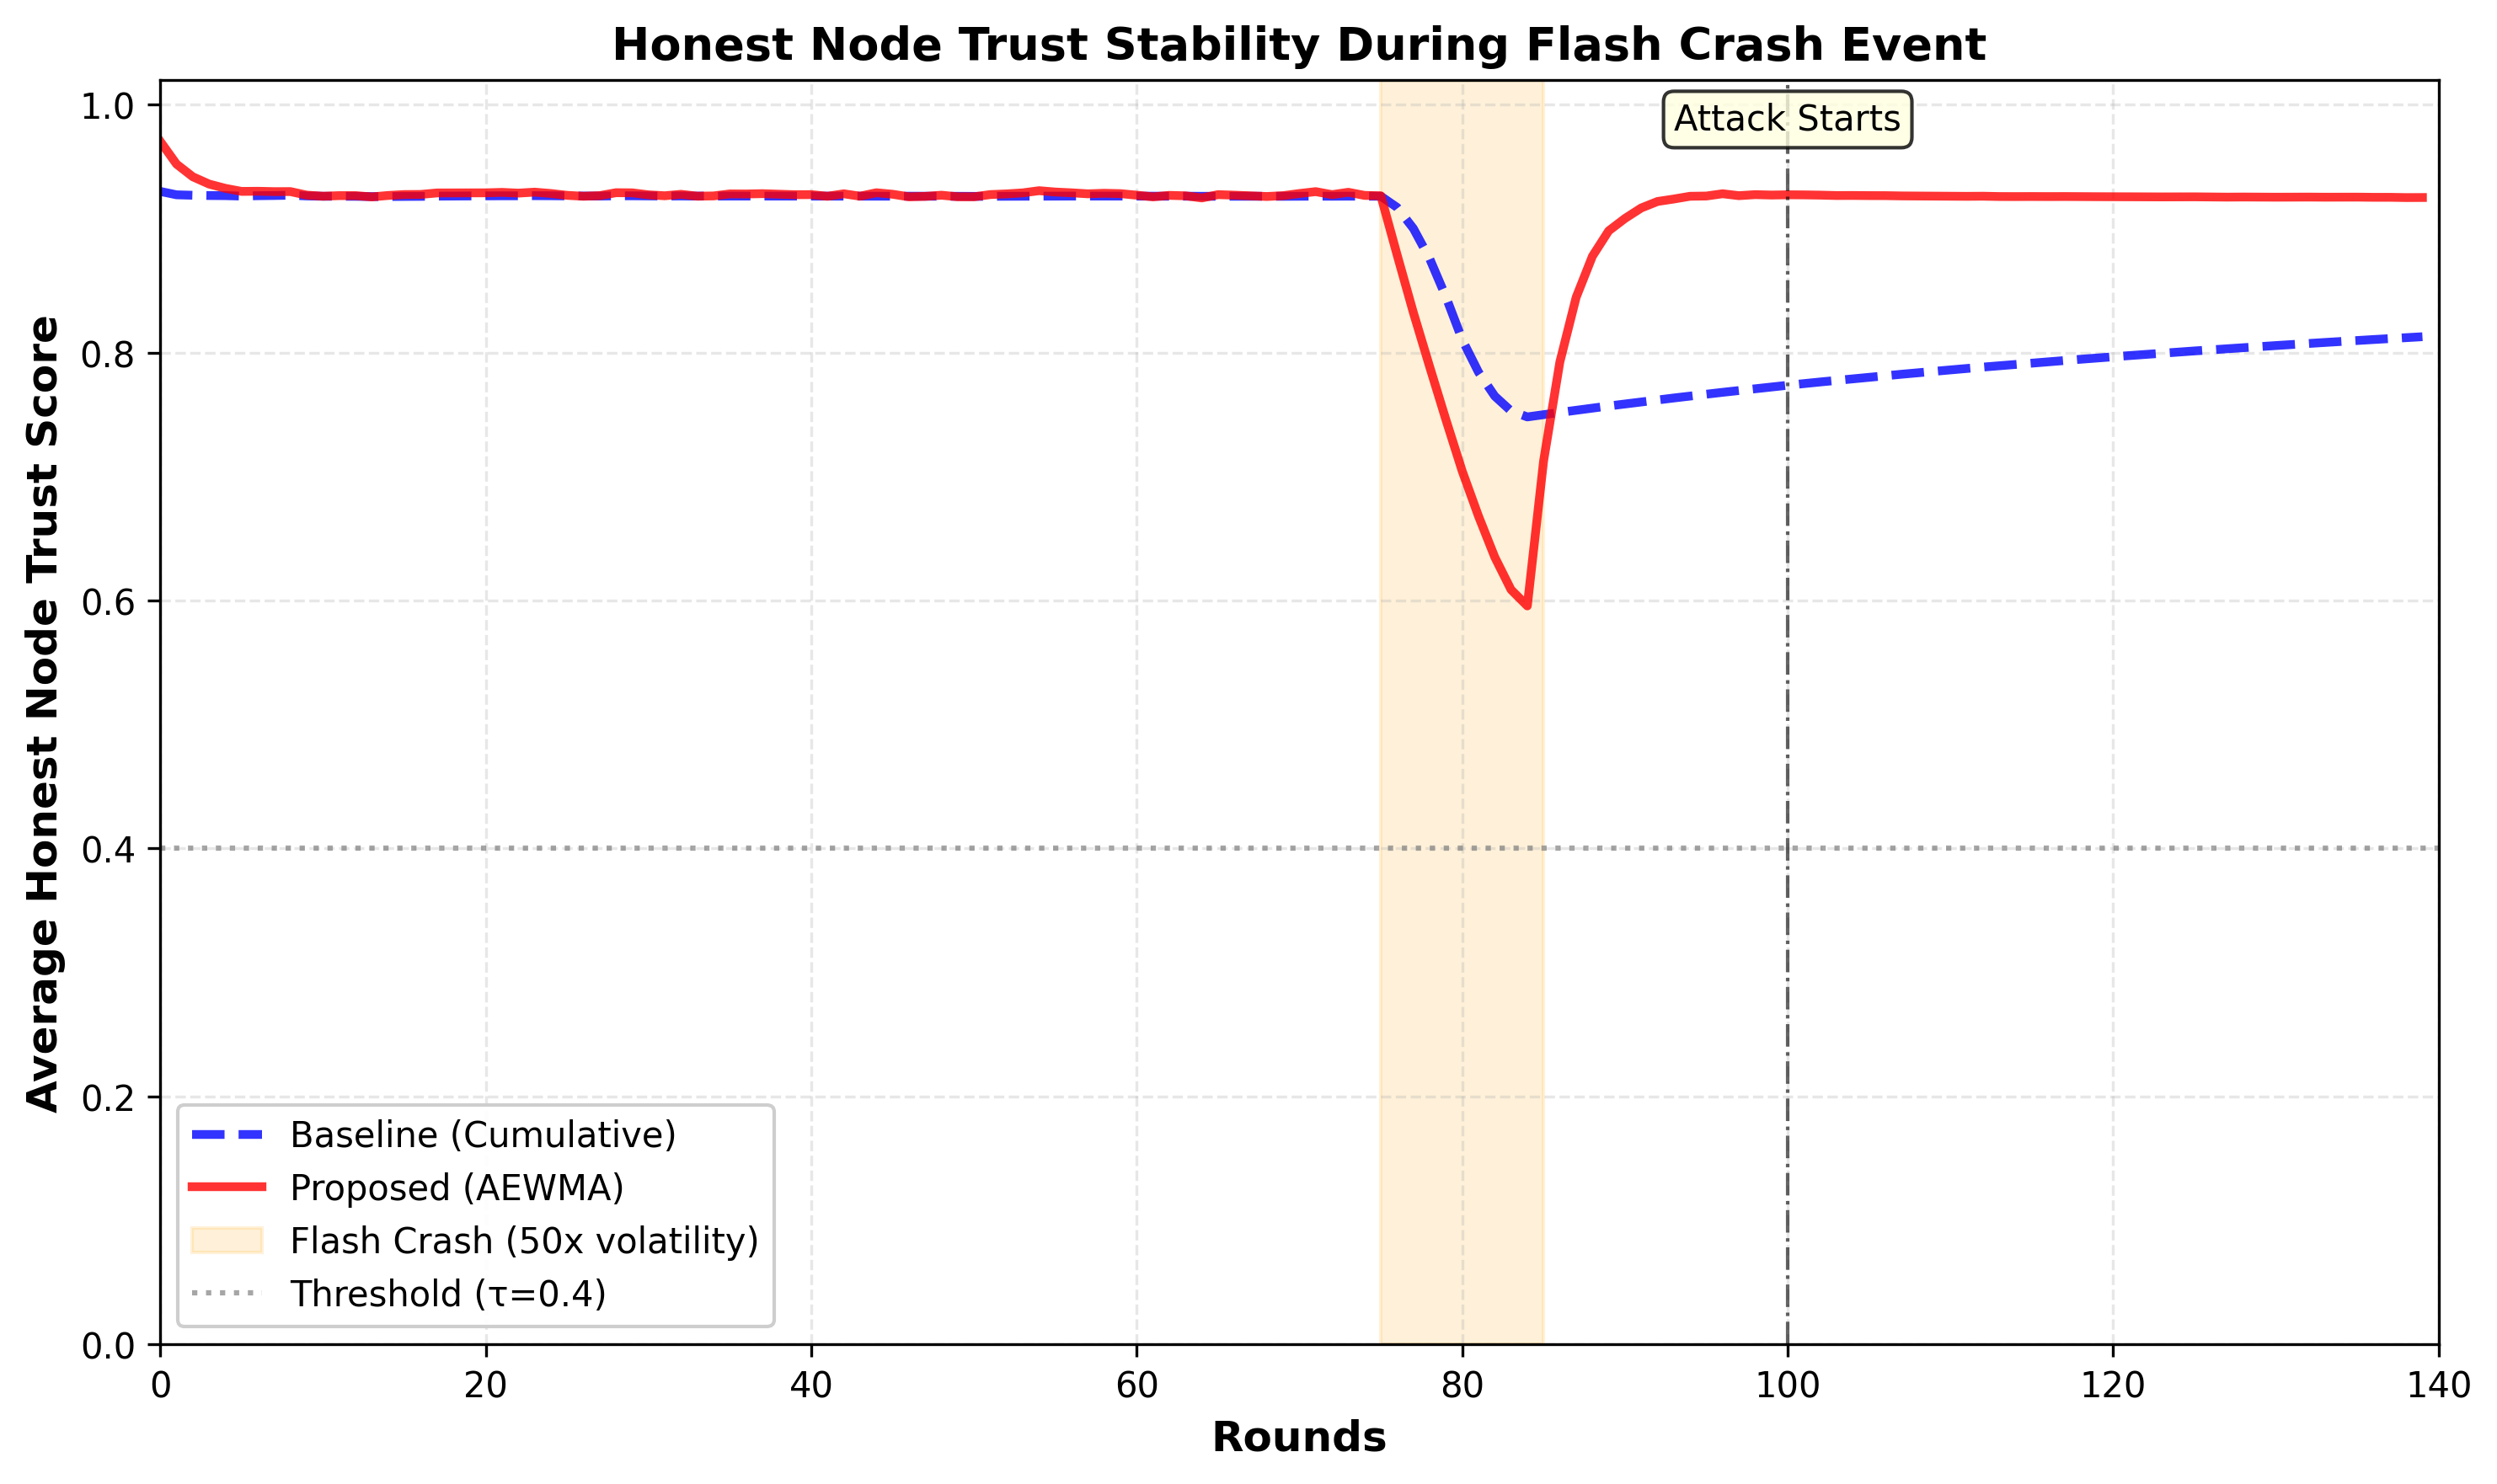
\includegraphics[width=\columnwidth]{Graph_5.png}
\caption{Honest Node Trust Stability During Flash Crash Event. A volatility spike (50$\times$) occurs at rounds 75--85 (orange region). Both methods dip during the crash, but the AEWMA (solid red) recovers to pre-crash trust levels within 5 rounds, while the static baseline (dashed blue) suffers permanent trust degradation that never fully recovers.}
\label{fig:stability}
\end{figure}

\subsection{Parameter Sensitivity Analysis}
\label{sec:sensitivity}
To quantify the influence of the sensitivity hyperparameter $\beta$ on system stability, we performed an extensive parameter sweep analysis across $\beta \in [0.1, 2.0]$ and volatility multipliers $\gamma \in [1\times, 5\times]$, visualized in the heatmap presented in Fig. \ref{fig:heatmap}. The heatmap was computed over 50 independent runs per ($\beta$, $\gamma$) configuration, totaling 5,000 simulation runs.

The results reveal three distinct operational regimes. First, the \textit{under-damped regime} ($\beta < 0.5$): low $\beta$ values produce insufficient volatility compensation, causing the system to behave similarly to the static baseline with elevated FPR at high volatility. Second, the \textit{optimal regime} ($\beta \approx 1.0$): at this value, the heatmap shows a ``safe zone'' (dark blue) where FPR remains near zero across all volatility levels, while still maintaining rapid attack detection. Third, the \textit{over-damped regime} ($\beta > 1.5$): excessively high $\beta$ values effectively suppress false positives across all conditions but introduce marginal latency in detecting active threats, as $\alpha_t$ becomes too small even during moderately volatile periods.

Therefore, we identified $\beta=1.0$ as the optimal equilibrium zone which provides a balanced robustness suitable for the volatility profiles of standard cryptocurrency assets. This value ensures that $\alpha_t$ drops below 0.1 only when network volatility exceeds $7\sigma_{normal}$, preserving attack detection capability under moderate market fluctuations.

\begin{figure}[!ht]
\centering
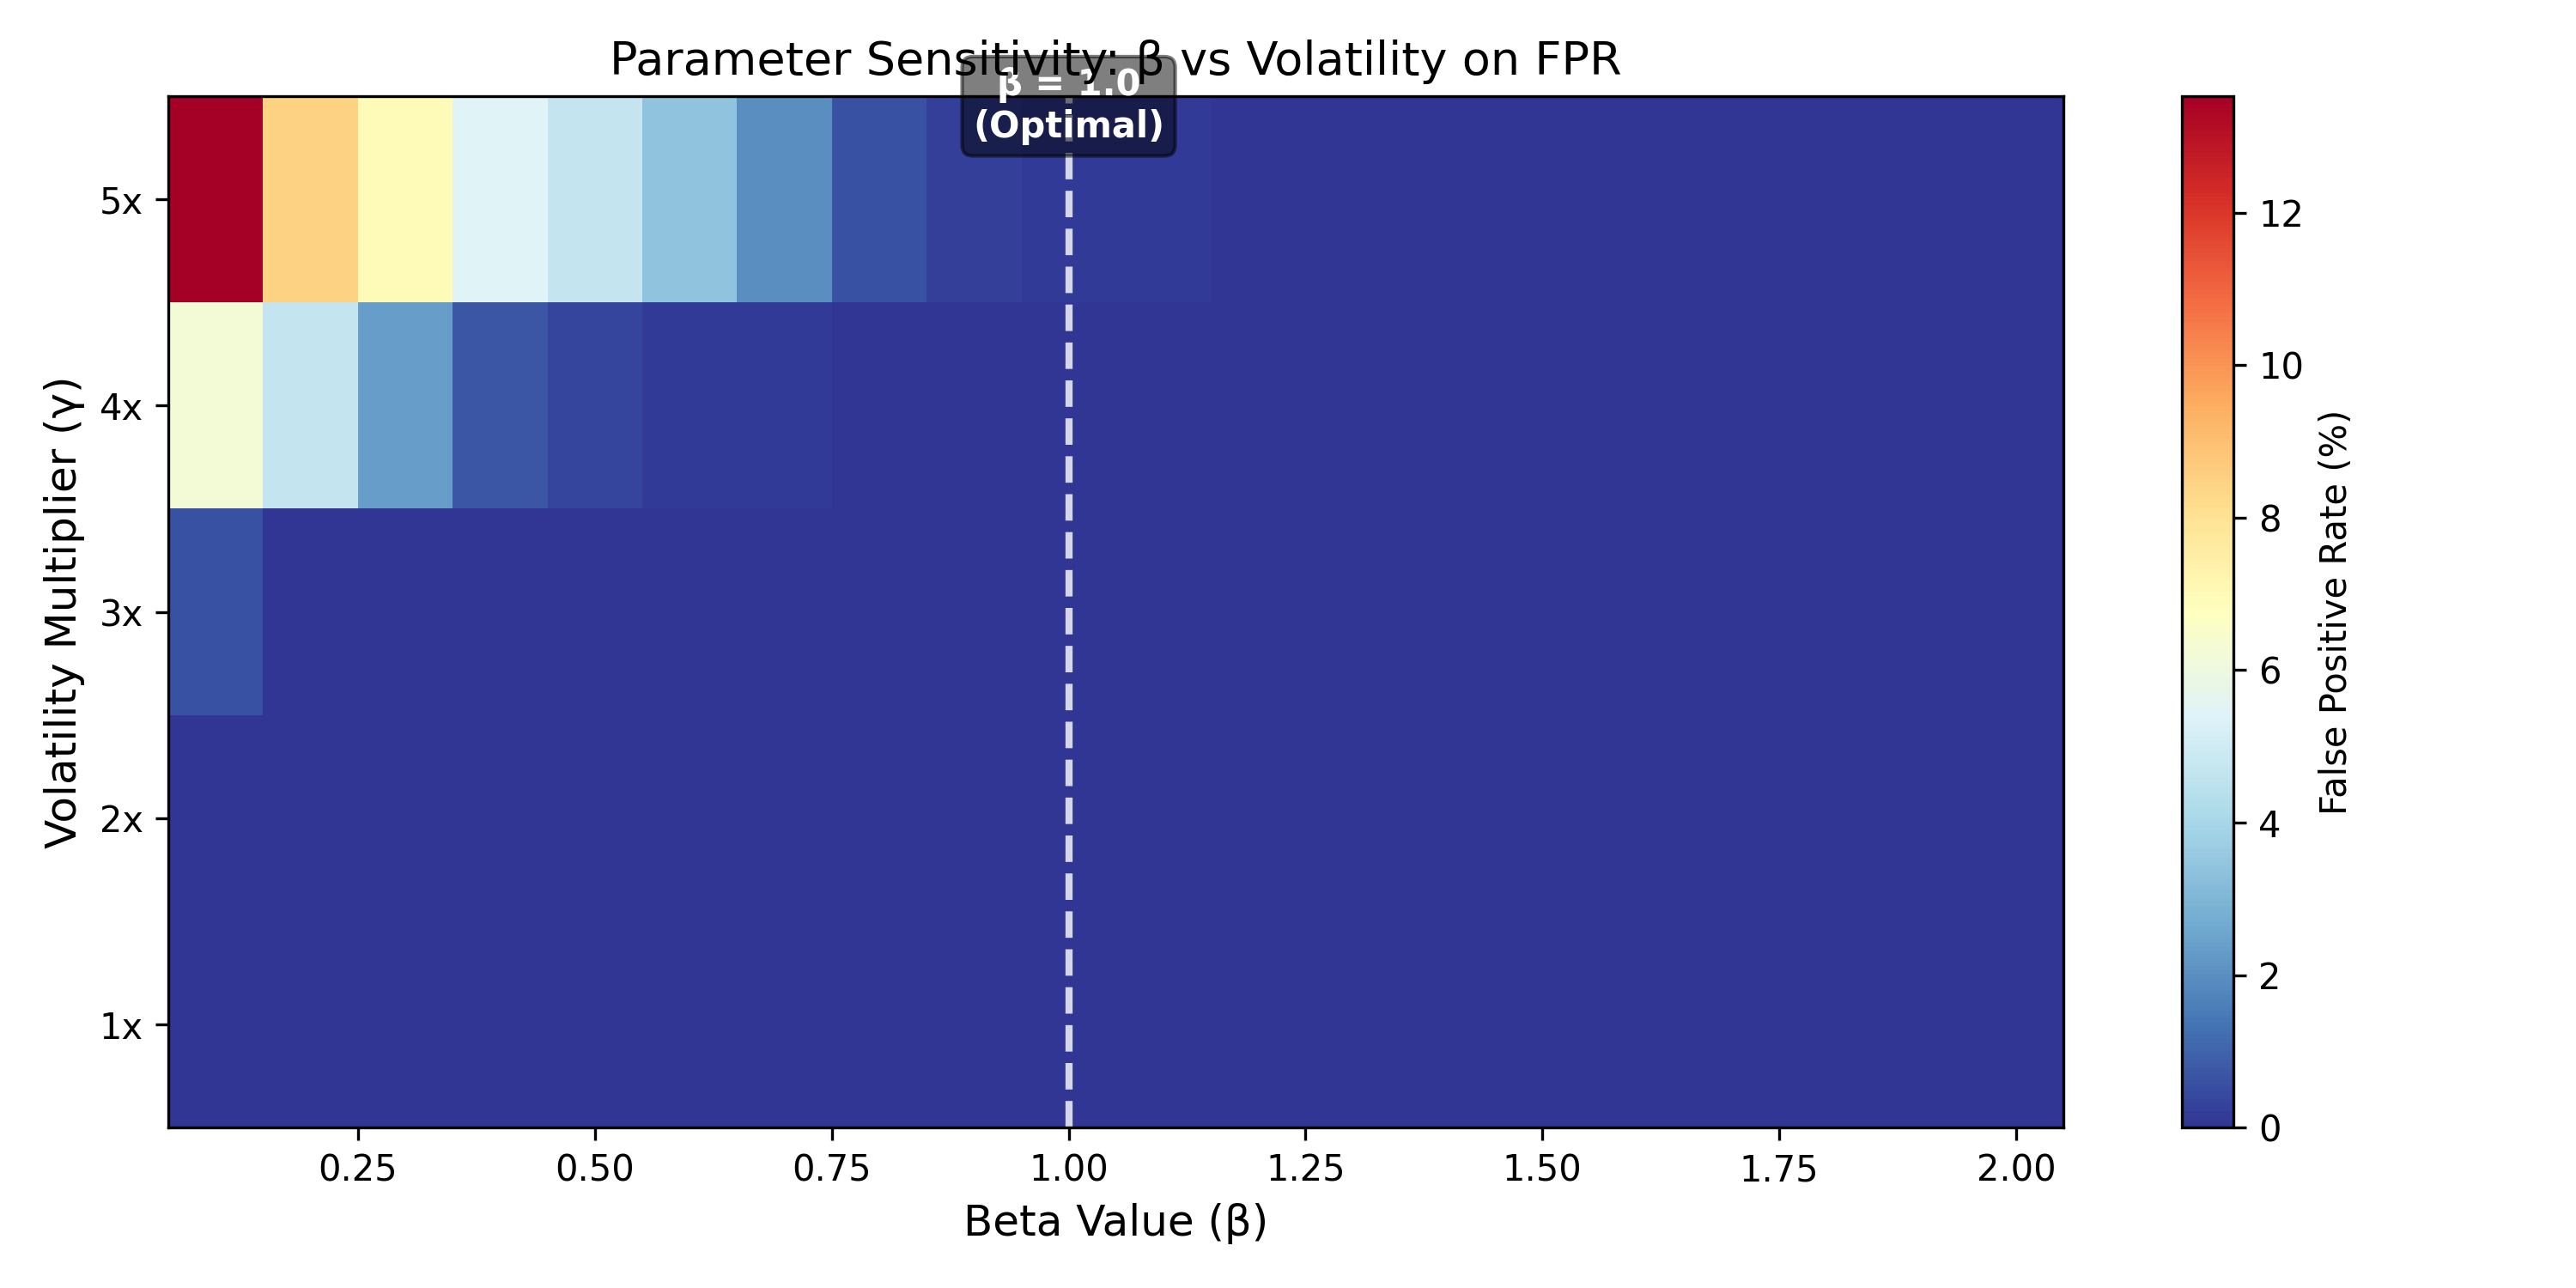
\includegraphics[width=\columnwidth]{Graph_3.png}
\caption{Sensitivity Analysis of $\beta$ vs. Volatility Multiplier. The heatmap shows FPR across 1,000 parameter configurations (50 runs each). The optimal zone at $\beta=1.0$ (white dashed line) maintains low FPR across all volatility levels. Low $\beta$ mirrors static behavior; high $\beta$ over-dampens detection.}
\label{fig:heatmap}
\end{figure}

% =====================================================================
\section{Discussion}
\label{sec:discussion}

\subsection{Gas Cost and Complexity Analysis}
A critical constraint for blockchain oracles is the execution cost (Gas). The traditional static graph approach often requires storing the entire history of interactions or computing cumulative sums, which can lead to integer overflow issues.

Our proposed AEWMA mechanism addresses this by minimizing state storage. As established in recent optimization studies \cite{b16}, storage operations (SSTORE) are the most expensive instructions in the Ethereum Virtual Machine (EVM), costing 20,000 gas for a new storage slot and 5,000 gas for updates. Our recursive formulation (Eq. \ref{eq:aewma}) satisfies the Markov property which means the next state depends only on the current state and current input:
\begin{equation}
\text{Storage}(AEWMA) \sim O(1) \text{ per edge}
\end{equation}
It only requires storing the most recent weight $w_{ij,t-1}$ and the current volatility state. This constant-space complexity makes the algorithm highly gas-efficient for on-chain implementation compared to sliding-window approaches that require $O(W)$ storage (where $W$ is the window size). Our Solidity implementation (Section \ref{sec:implementation}) demonstrates this with packed storage keys, reducing the total SSTORE operations to $O(N^2)$ per round with each operation being a simple arithmetic update.

\subsection{Scalability and Off-Chain Computation}
Although the pairwise weight update is $O(1)$, the graph construction scales at $O(N^2)$ due to the pairwise comparisons between all oracles. For small permissioned networks (e.g., $N \le 20$), this is computationally feasible on-chain, as demonstrated by our Solidity implementation which processes 20 nodes within reasonable gas limits.

However, for larger decentralized networks, the $O(N^2)$ complexity presents a scalability bottleneck \cite{b17}. To address this, we propose a hybrid architecture (depicted in the right portion of Fig. \ref{fig:architecture}): the graph generation and Maximum Independent Set (MIS) extraction are performed off-chain with the results and cryptographic proofs submitted on-chain. The trust decay logic can then be applied as a lightweight verification layer on the smart contract to validate the submitted consensus. This hybrid approach allows the protocol to scale without incurring heavy on-chain computation costs.

\subsection{Resilience to Flash Crash Events}
The results presented in Fig. \ref{fig:stability} reveal an important insight about the temporal dynamics of trust management. While both the AEWMA and static methods experience trust disruption during a flash crash event, the AEWMA's \textit{adaptive forgetting} property provides a critical advantage: automatic recovery. In traditional systems, a single flash crash event can permanently degrade the trust scores of honest nodes, requiring manual intervention or system reset. The AEWMA's fading memory naturally purges the crash-induced noise once market conditions normalize, restoring the network to its pre-crash operational state. This self-healing property is essential for autonomous oracle systems that must operate continuously without human oversight.

\subsection{Sybil Resistance Limitations}
It is important to note that while our graph-based profiling effectively isolates malicious clusters, it relies on the assumption that the largest clique in the graph consists of honest nodes. As proven in the foundational work on Sybil attacks \cite{b10}, no reputation system can fully eliminate Sybil actors without either a central identity authority or significant economic barriers. Therefore, our ``Incentive Compatibility'' (Section IV.D) is a necessary companion to the graph logic. The staking requirement in our Solidity implementation provides this economic barrier, making it costly for attackers to create multiple identities.

\subsection{Comparison with State-of-the-Art}
Table \ref{tab:comparison} summarizes the key advantages of the proposed approach over existing methods. Unlike voting-based systems, our method captures pairwise behavioral patterns. Unlike static graph-based methods \cite{b7}, our approach adapts to environmental conditions and provides a complete on-chain implementation. The combination of volatility-aware trust decay with economic incentive compatibility (slashing) creates a comprehensive defense against both strategic attacks and environmental disruptions.

% =====================================================================
\section{Conclusion}
\label{sec:conclusion}
In this paper, we identified and formalized the problem of Reputation Inertia in graph-based blockchain oracles, where accumulated history masks recent malicious behavior (Whitewashing) and environmental volatility triggers false positives (Flash Crashes).

We proposed a novel dynamic profiling mechanism based on an Adaptive Exponential Weighted Moving Average (AEWMA). By modulating the learning rate $\alpha_t$ via real-time network volatility, our system is hypersensitive to attacks during stability and robust to noise during volatility. We provided a complete Solidity smart contract implementation demonstrating the on-chain feasibility of the mechanism with $O(1)$ storage per edge weight. Through extensive Monte Carlo simulations (100 runs) using a 20-node oracle network with historical cryptocurrency price dynamics, we demonstrated that the proposed method reduces the average Time-to-Detection for whitewashing attacks from 9.0 rounds (static baseline) to 1.7 rounds, representing an 81\% improvement. Simultaneously, the AEWMA mechanism maintained a False Positive Rate of only 0.4\% under extreme volatility conditions ($5\times$ standard deviation), compared to 7.1\% for the static approach. The flash crash stability analysis further demonstrated that AEWMA achieves self-healing trust recovery within 5 rounds of crash termination, while static methods suffer permanent trust degradation. Parameter sensitivity analysis confirmed that $\beta=1.0$ provides the optimal trade-off between detection speed and false positive suppression across varying market conditions. Future work will focus on integrating this reputation model with Zero-Knowledge Proofs (ZKPs) to allow for fully private and scalable on-chain reputation verification, and extending the evaluation to larger-scale networks with heterogeneous adversarial strategies.

% References
\bibliographystyle{IEEEtran}
\bibliography{references}

\EOD

\end{document}
